\chapter{Theoretical Approach}

\section{Setup}

For the theoretical approach we consider a $1km$ long highway in Switzerland. The cars with a average weight of $1302 kg $ or $12772 N$ travel over this road. We estimate the wheel of the cars to have an average width of $22cm$ and an area of $0.0352m^2$ ground contact since the part of the wheel which touches the ground is about $4cm$ long.\cite{Kim2023}\\
In total, there will be $100000$ Piezoelectric elements connected in series planted into the road of size $22 \times 4 cm$ and a thickness of $0.133mm$ which was calculated by calculating the force needed to achieve $10 V$ with the piezoelectric element in the experiment. Afterwards the force was devided by the weight force of the car to get the constant by how much the the thickness had to be increased.
$$
F = \frac{10 \cdot 0.0088}{21.3 \cdot 10^{-3} \cdot 0.00022} = 21050 N
$$
$$
\frac{12772}{21050} = 0.6
$$
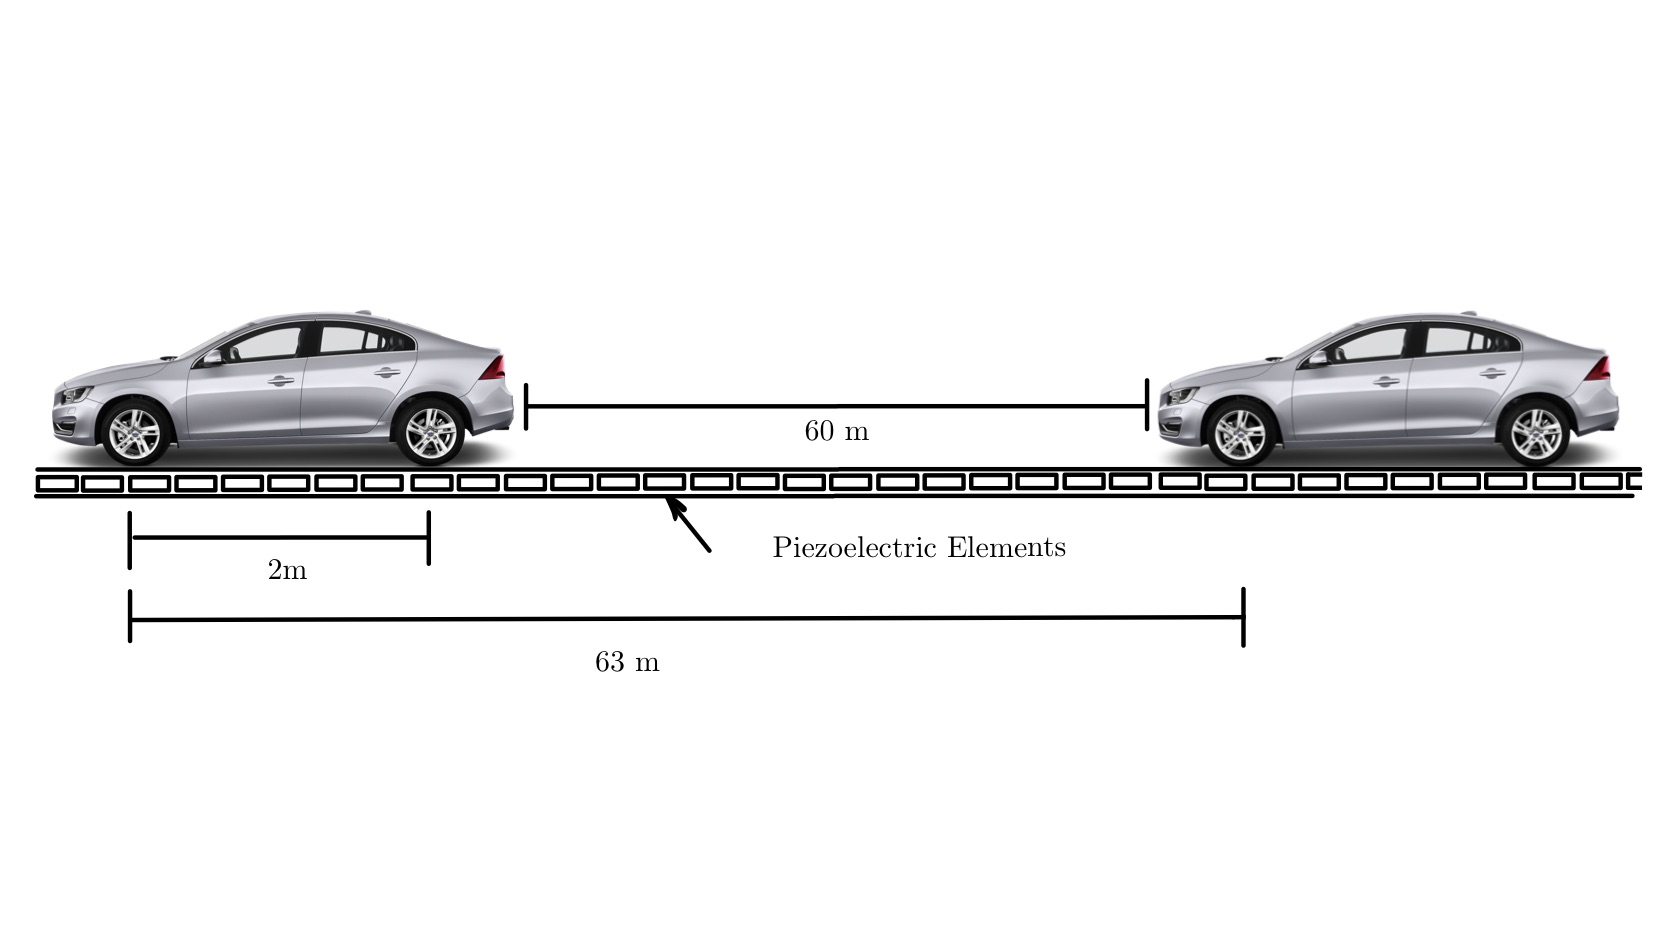
\includegraphics[width=\textwidth]{Figure_13.jpg}
\captionof{figure}{Setup of the Theoretical Approach}
\label{fig:Setup of Theoretical Approach}
\vspace{0.5cm}
A car is about $3m$ long in average and on the highway the cars have a distance of $60m$. Considering the fact that the wheels have a distance of $0.5m$ from the nose and tail of the car, the distance of the front wheel of the car infront will be $63m$ from the front wheel in the car in the back. (Figure \ref{fig:Setup of Theoretical Approach})\\

\section{Calculations}

So in an ideal scenario 15 cars can fit onto a $1km$ long road but not all of them have driven over the piezoelectric elements which also counts for the wheels. For the car in front only the front wheels have driven over all piezoelectric elements. The back wheels have driven over all except the last 100. This continues on for the next few cars.\\
This leads to the formula $2 \cdot \sum_{i=0}^{15} 4.51 \cdot (50000 - (i\cdot 1575)) + 4.51 \cdot (49900 - (i \cdot 1575))$ for the voltage since $V = 23.2 \cdot 10^{-3} \cdot \frac{12772 \cdot 0.000133}{0.0088} = 4.51V$, the amount of piezoelectric elements which the back wheels don't cover is 100, and the number of piezoelectric elements which the front wheels of the car in the back don't cover is 1575. In addition, there are two lanes hence we have to multiply the sum by 2. This leads to a output voltage of $11MV$.\\
For the energy, we can replace the voltage by the energy which is $E = \frac{1}{2} \cdot 1302 \cdot 9.81 \cdot \frac{1302 \cdot 9.81}{10^{10}} = 0.0081J = 2.27 \mu Wh$. This leads to $2 \cdot \sum_{i=0}^{15} 2.27 \cdot 10^{-6} \cdot (50000 - (i\cdot 1575)) + 2.27 \cdot 10^{-6} \cdot (49900 - (i \cdot 1575)) = 4.7Wh$